\documentclass{article}

%other packages
\usepackage[a4paper, total={7.5in, 10.5in}]{geometry}
\usepackage{longtable}
\usepackage{wrapfig}
\setlength\parindent{0pt}
\usepackage{enumitem}
\usepackage[table]{xcolor}
\usepackage{polynom}

%maths
\usepackage{mathtools}
\usepackage{amsmath}
\usepackage{amssymb}
\usepackage{amsfonts}
\usepackage{autobreak}

%tikzpicture
\usepackage{tikz}
\usepackage{scalerel}
\usepackage{pict2e}
\usepackage{tkz-euclide}
\usetikzlibrary{calc}
\usetikzlibrary{patterns,arrows.meta}
\usetikzlibrary{shadows}
\usetikzlibrary{external}

%pgfplots
\usepackage{pgfplots}
\pgfplotsset{compat=newest}
\usepgfplotslibrary{statistics}
\usepgfplotslibrary{fillbetween}
\usepgfplotslibrary{polar}

\pgfplotsset{
    standard/.style={
    axis line style = thick,
    trig format=rad,
    enlargelimits,
    axis x line=middle,
    axis y line=middle,
    enlarge x limits=0.15,
    enlarge y limits=0.15,
    every axis x label/.style={at={(current axis.right of origin)},anchor=north west},
    every axis y label/.style={at={(current axis.above origin)},anchor=south east}
    }
}

\begin{document}

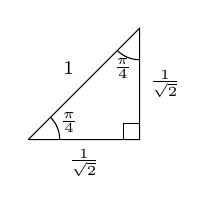
\begin{tikzpicture}[scale=2]
    \coordinate (A) at (0,0);
    \coordinate (B) at (45:1);
    \coordinate (C) at (45:1|-0,0);
    \draw (A)--node[pos=0.5,above left]{$\scriptstyle1$}(B)--node[pos=0.5,right]{$\scriptstyle\frac{1}{\sqrt{2}}$}(C)--node[pos=0.5,below]{$\scriptstyle\frac{1}{\sqrt{2}}$}(A);
    \draw pic["$\scriptstyle\frac{\pi}{4}$",draw,-,angle eccentricity=1.4, angle radius=0.4cm]{angle=C--A--B};
    \draw pic["$\scriptstyle\frac{\pi}{4}$",draw,-,angle eccentricity=1.4, angle radius=0.4cm]{angle=A--B--C};
    \draw pic[draw,-,angle eccentricity=1.4, angle radius=0.2cm]{right angle=B--C--A};
\end{tikzpicture}
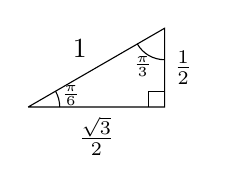
\begin{tikzpicture}[scale=2]
    \coordinate (A) at (0,0);
    \coordinate (B) at (30:1);
    \coordinate (C) at (30:1|-0,0);
    \draw (A) -- node[pos=0.5,above left]{$1$} (B) -- node[pos=0.5,right]{$\frac{1}{2}$} (C) -- node[pos=0.5,below]{$\frac{\sqrt{3}}{2}$} (A);
    \draw pic["$\scriptstyle\frac{\pi}{6}$",draw,-,angle eccentricity=1.4, angle radius=0.4cm]{angle=C--A--B};
    \draw pic["$\scriptstyle\frac{\pi}{3}$",draw,-,angle eccentricity=1.4, angle radius=0.4cm]{angle=A--B--C};
    \draw pic[draw,-,angle eccentricity=1.4, angle radius=0.2cm]{right angle=B--C--A};
\end{tikzpicture}

\end{document}
